\documentclass[letterpaper, 12pt]{article}
\usepackage[letterpaper, top=2.5cm, bottom=2.5cm, left=3cm, right=3cm]{geometry} %margenes
\usepackage[backend=biber]{biblatex}\addbibresource{bibliografia.bib} %manejo de bibliografía (BORRAR SI NO ES NECESARIO)
\usepackage[utf8]{inputenc} %manejo de caracteres especiales
\usepackage[spanish]{babel} %manejo de encabezados de inglés a español
\usepackage{fancyhdr} %formato de los encabezados de página
\usepackage{ragged2e} %alineado real justficado
\usepackage{graphicx} %manejo de imagenes
\usepackage{amsmath} %manejo de notación matemática
\usepackage{mathtools} %manejo de notación matemática
\usepackage{blindtext} %texto de relleno
\usepackage{amssymb} %manejo de simbología
\usepackage{float} %centrado de imaene
\usepackage{hyperref} %manejo de enlaces e hipervínculos

\hypersetup{
  colorlinks   = true, %Colours links instead of ugly boxes
  urlcolor     = blue, %Colour for external hyperlinks
  linkcolor    = blue, %Colour of internal links
  citecolor   = red %Colour of citations
}

\pagestyle{fancy}
\fancyhf{}
\rfoot{\thepage}

\nocite{*}

\begin{document}
    
    %PORTADA
    \begin{titlepage}
        \begin{figure}[ht]
            \centering
            
\includegraphics[width=15cm]{logosITT.png}
        \end{figure}
        \centering
        {\scshape\LARGE Tecnológico Nacional de México\\Instituto Tecnológico de Tijuana\par}
        \vspace{1cm}
        {\scshape\Large Arquitectura de Computadoras\par}
        \vspace{1cm}
        {\scshape\Large Unidad 1\par}
        \vspace{1.5cm}
        {\huge\bfseries Análisis de los componentes (CPU)\par}
        \vspace{2cm}
        {\Large\itshape C. Abraham Jhared Flores Azcona\\19211640\par}
        \vfill
        Profesor: M.C. Adrian Silva Ramirez\par
    
        \vfill

        {\large 1ro. de marzo de 2021}
    \end{titlepage}

    %indice
    \newpage
        \thispagestyle{empty}
        \tableofcontents
        \listoffigures

    %cuerpo
    \newpage
    \begin{justify}
        \setcounter{page}{1}
        \thispagestyle{fancy}
        \lhead{\textbf{Análisis de los componentes (CPU)}}
        \section{Introducción}
        \justify
        Como parte del conocimiento de la asignatura, es de vital importancia conocer los componentes para tener un mejor entendimiento 
        de la función de una computadora. En esta breve investigación se habla del CPU y las tecnicalidades necesarias para las competencias de la materia.
        \section{CPU}
        \justify
        Esta es la unidad central de procesamiento (por sus siglas en inglés), tambien referido de manera coloquial como ``el corazón'' ó ``el cerebro'' de la computadora.
        De manera concreta, el CPU toma las instrucciones de un programa o aplicación y realia un cálculo. Dicho proceso se separa en cuatro momentos clave:
        \[\textbf{Fetch}\rightarrow\textbf{Decode}\rightarrow\textbf{Execute}\rightarrow\textbf{Store}\]
        El proceso toma la entrada de un dispositvo periferico ó de un programa de computadora e interpreta lo necesario para que el CPU exprese la tarea requerida del periferico ó poder
        deplegarlo en el monitor. Se representa de la siguiente manera:
        \begin{figure}[H]
            \centering
            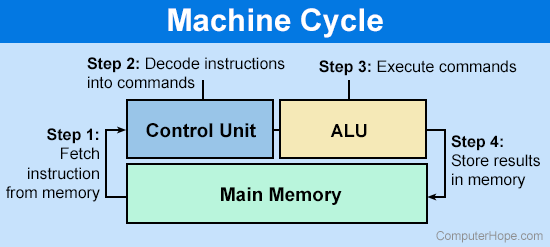
\includegraphics[width=10cm]{cycle.png}
            \caption{Modelo del ciclo de maquina en un CPU.}
        \end{figure}
        \subsection{Arquitecturas}
        \justify
        Se les llama \emph{microarquitecturas}. Por fines de brevedad, se explican dos arquitecturas comunmente mencionadas: \emph{ARM y x86}.
        \subsubsection*{ARM}
        \justify
        Construidos en base al modelo RISC (\emph{reduced instruction set computer}) desarrollado por Advanced RISC Machines (ARM).
        \\\newline
        Son usados de manera extensiva en dispositivos eletrónicos de consumo como smartphones, tabletas, reproducores multimedia y otros. Debido a su conjunto de instrucciones reducido, requieren
        pocos transistores, lo que permite un tamaño de pastilla pequeño para el circuito integrado. El tamaño menor del procesador ARM, su complejidad reducida y menor consumo de energía hacen a estos procesadores 
        capaces para ser empleados en dispositivos en constante miniaturización.
        \\\newline
        Las características de los procesadores ARM incluyen:
        \begin{itemize}
            \item Arquittecura de carga/almacenamiento.
            \item Un conjunto de instrucciones ortogonales.
            \item Ejecución de un solo ciclo.
            \item Diseño ahorrador de energía.
            \item Estados de ejecución de 64 y 32 bits para rendimieno escalable.
            \item Soporte de virtualización de hardware.
        \end{itemize}
        \begin{figure}[H]
            \centering
            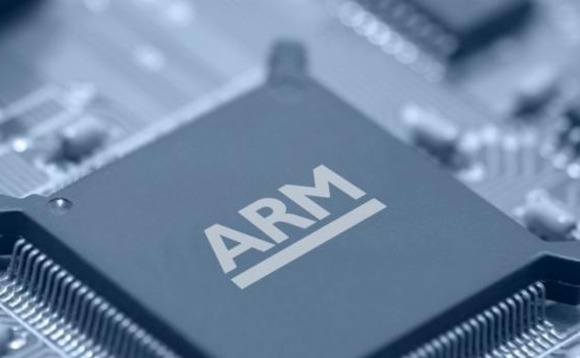
\includegraphics[width=8cm]{arm.jpeg}
            \caption{Imágen alusiva de un CPU con arquitectura ARM.}
        \end{figure}
        \subsubsection*{x86}
        \justify
        La linea más exitosa de procesadores Intel. Desarrollado en base al microproceador Intel 8086 de 16 bits. El termino actualmente se usa para referirse a cualquier microproceador de 32 bits
        compatible con el conjunto de instrucciones x86. Dicha arquitectura maneja principalmente funciones programables y provee servicios, tale como direcciones de memoria, manejo de interrupciones de software y hardware,
        tipos de dato, manejo de registros y de dispositivos de entrada y salida.
        \\\newline
        Sus caracteristicas principales incluyen:
        \begin{itemize}
            \item Provee de un marco de trabajo lógico para ejecutar instrucciones a travéz de un procesador.
            \item Permite a programas e instrucciones para ejecutar en cualquier procesador en la familia Intel 8086.
            \item Provee procedimientos para utilizar y administrar los componentes físicos de un CPU.
        \end{itemize} 
        \begin{figure}[H]
            \centering
            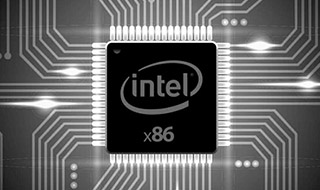
\includegraphics[width=8cm]{x86.jpg}
            \caption{Imágen alusiva de un CPU con arquiectura x86.}
        \end{figure}

        \subsection{Tipos}
        \justify
        Los distintos tipos de los proceadores se construyen con arquitecturas de 64 bits y 32 bits con velocidad máxima y capacidad flexible. Para generalizar, los tipos de CPU populares son clasificados
        en \emph{un núcleo}, \emph{dos núcleos}, \emph{cuatro núcleos}, \emph{ocho núcleos}, \emph{diéz núcleos}.
        \subsubsection*{Un núcleo}
        \justify
        El tipo más viejo empelado en computadoras personales. Solo puede ejecutar un solo comando a la vez y no es eficiente en multi-tareas.
        \subsubsection*{Dos núcleos}
        \justify
        Es un solo CPU que se compone de dos núcleos que se comportan como uno. Puede manejar multitareas. No e muy robusto como un CPU de cuatro núcleos. 
        \subsubsection*{Cuatro núcleos}
        \justify
        Cuatro núcleos en un solo CPU. Utilizado por personas que necesitan múltiples programas al mismo tiempo.
        \subsubsection*{Seis núcleos}
        \justify
        Encontrados en celulares inteligentes de última generación.
        \subsubsection*{Ocho núcleos}
        \justify
        Consiste en un conjunto dual de procesadores de cuatro núcleos.
        \subsubsection*{Diéz núcleos}
        \justify
        Consiste en cuatro conjuntos de cuatro núcleos y seis conjuntos de seis núcleos. La mejor opción en contraste a otros tipos.

        \subsection{Características}
        \justify
        Aquí se explican de manera breve las características más recientes para los procesadores.
        \subsubsection*{Manufacturador del procesador y su modelo}
        \justify
        Esto refiere a quien hizo el procesador y el modelo. Debido a que los procesadores de las compañias tienden a ser muy similares en rendimiento,
        no se puede instalar un procesador AMD en una tarjeta madre compatible con procesadores Intel y viceversa.
        \subsubsection*{Tipo de enchufe}
        \justify
        El enchufe al cual fue hecho apra encajar. Llegara el caso de que se remplazara un CPU con otro, el reemplazo debe de poder encajar con el enchufe del anterior.
        \subsubsection*{Velocidad de reloj}
        \justify
        Especificado en megahertz (\(MHz\)) o gigaherts (\(GHz\)). Esta característica determina el rendimiento. Usado para mantener estándares dentro de las compañias para
        medir los rendimientos de sus CPU's.
        \subsubsection*{Velocidad \emph{Host-bus}}
        \justify
        Especifíca la razón de transeferencia de datos entre el procesador y el chipset. Mientras más rápida esta característica, contribuye a un rendimiento mayor del procesador, aún
        para procesadores que manejen la misma velocidad de reloj.
        \subsubsection*{Tamaño de la memoria cache}
        \justify
        Como se indica, que tan grande es la memoria principal. Para algunas aplicaciones particulares que operan en conjuntos de datos pequeños, mayor memoria cache aumenta la velocidad del procesador,
        epecialmente en modelos Intel.
        \subsubsection*{Tamaño del procesador}
        \justify
        Indica el tamaño de los elementos individuales más pequeños en la pastilla del procesador.  Esto importa ya que un procesador que usa componentes más pequeños puede funcionar más rápido, usar menor voltaje,
        consumir menos energía y producir menos calor.

        \subsection{Funcionamiento (ALU, Unidad de control, Registros y buses internos)}
        \justify
        La arquitectura de un CPU comúnmente se ilustra de la siguiente manera:
        \begin{figure}[H]
            \centering
            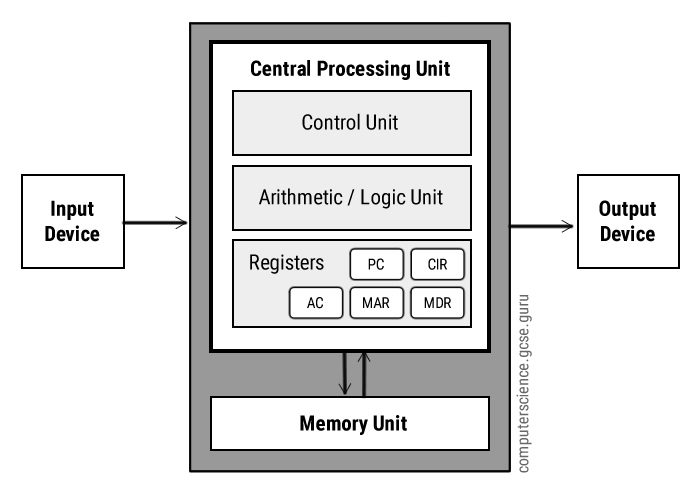
\includegraphics[width=10cm,height=7cm]{CPU.jpg}
            \caption{Modelo de la arquitectura Von-Neumann para un CPU.}
        \end{figure}
        \justify
        En la imágen se aprecia en la \emph{Central Processing Unit} sus componentes que son los del subtema en cuestión.
        \subsubsection*{ALU}
        \justify
        Unidad Aritmética-Lógica. Permite que las operaciones lógicas y aritméticas puedan realizare.
        \subsubsection*{Unidad de control}
        \justify
        Como su nombre lo indíca, controla las operaciones del ALU, a la memoria principal y a los dispositivos de entrada y salida
        y les indica como responder a la instrucción del programa que acaba de leer e interpretar.
        \subsubsection*{Registros}
        \justify
        Son areas de almacenamiento velóz en el CPU. Todos los datos deben de ser almacenados en estos registros antes de que sean proceados.
        Dicho registros son los siguientes:
        \begin{itemize}
            \item \textbf{MAR (Registro de la dirección de memoria):} Mantiene la localización de memoria de los datos que deben de ser accesados.
            \item \textbf{MDR (Registro de los datos de memoria):} Mantiene los datos que están siendo transferidos hacia o desde la memoria.
            \item \textbf{AC (Acumulador):} Donde los reultados de aritmético y lógica son almacenados.
            \item \textbf{PC (Contador del programa):} Contiene la dirección de la siguiente instrucción a ser ejecutada.
            \item \textbf{CIR (Registro de la instrucción actual):} Contiene la instrucción actual en el procesamiento.
        \end{itemize}
        \subsubsection*{Buses internos}
        \justify
        Son los medios por los cuales los datos on transmitidos de una parte de la computadora a otra, conectando todos los componente internos con el CPU y la memoria.
        \\\newline
        Un CPU estándar está compuesto por los siguientes buses:
        \begin{itemize}
            \item \textbf{Bus de control}: Lleva consigo las direcciones de datos (pero no los datos en sí) entre el procesador y la memoria.
            \item \textbf{Bus de datos}: LLeva consigo los datos entre el procesador, la unidad de memoria y los dispositivos de entrada y de salida.
            \item \textbf{Bus de control}: LLeva consigo comandos entre el CPU (y otros comandos de otros dispositivos) en orden para controlar y coordinar todas las actividades entre la computadora.
        \end{itemize}
        \section{Conclusión}
        \justify
        Como todo sistema, el conocer las tecnicalidades de una de las partes más relevantes de un equipo de cómputo permite aumentar el conocimiento del mismo para aprovechar este componente
        al máximo.

    \end{justify}

    %formato de página de bibliografía
    \fancypagestyle{justanumber} %estilo personalizado para la bibliografia
    {
        \fancyhf{}
        \renewcommand\headrulewidth{0pt}
        \renewcommand\footrulewidth{0pt}
        \fancyfoot[R]{\thepage}
    } %sin la barrita ni los encabezados, solo el numero de página en el pie derecho

    %bibliografía
    \newpage
        \thispagestyle{justanumber}
        \addcontentsline{toc}{section}{Referencias}
        \printbibliography

\end{document}